\documentclass[12pt,a4paper]{article}
\usepackage[utf8]{inputenc}
\usepackage[margin=1in]{geometry}
\usepackage{amsmath}
\usepackage{amsfonts}
\usepackage{amssymb}
\usepackage{graphicx}
\usepackage{listings}
\usepackage{xcolor}
\usepackage{fancyhdr}
\usepackage{titlesec}
\usepackage{tikz}
\usetikzlibrary{positioning,shapes,arrows}
\usepackage[colorlinks=true, linkcolor=blue, urlcolor=blue, citecolor=blue]{hyperref}


% SQL syntax highlighting
\lstdefinestyle{sqlstyle}{
    language=SQL,
    basicstyle=\ttfamily\small,
    keywordstyle=\color{blue}\bfseries,
    commentstyle=\color{green!50!black},
    stringstyle=\color{red},
    numbers=left,
    numberstyle=\tiny\color{gray},
    numbersep=5pt,
    breaklines=true,
    breakatwhitespace=true,
    tabsize=2,
    showspaces=false,
    showstringspaces=false,
    frame=single,
    rulecolor=\color{gray!30},
    backgroundcolor=\color{gray!5}
}

\lstset{style=sqlstyle}

% Page setup
\pagestyle{fancy}
\fancyhf{}
\rhead{CSE 414 - Assignment 04}
\lhead{Oracle SQL Practice}
\cfoot{\thepage}

% Title formatting
\titleformat{\section}{\Large\bfseries}{}{0em}{}
\titleformat{\subsection}{\large\bfseries}{}{0em}{}

\begin{document}

% Title Page
\begin{titlepage}
    \begin{figure}[htbp]
    \centering
    
\includegraphics[width=0.2\textwidth]{cu.png}
    \end{figure}
    \centering
    \vspace*{0.5cm}
    {\Huge\bfseries University of Chittagong}\\[0.5cm]
    {\Large Department of Computer Science \& Engineering}\\[0.5cm]
    {\large Database Systems Lab}\\[2cm]
    
    {\large Name of the assignment:}\\[0.3cm]
    {\LARGE\bfseries Database Modeling: Mini Project 1\\[0.5cm]}
    {\large CSE 414}\\[0.5cm]
    {\large Assignment 05}\\[3cm]
    
    \begin{minipage}[t]{0.4\textwidth}
    \raggedleft
    Submitted By:\\
    \large \textbf{Debashish Chakraborty}\\
    \large ID: 23701034
    \end{minipage}
    \hspace{0.05\textwidth}
    \vrule width 1pt
    \hspace{0.05\textwidth}
    \begin{minipage}[t]{0.4\textwidth}
    Submitted To:\\
    \large \textbf{Dr. Rudra Pratap Deb Nath}\\
    \large Associate Professor
    \end{minipage}
    
    \vfill
    {\large June 22, 2025}
\end{titlepage}

\newpage
\tableofcontents
\newpage 

\section{Introduction}

The requirements of this mini-project is to create and work with a medical database. The first step is to identify the information that is going to be represented in a database model. The information is modeled in an ER diagram and mapped to a relational schema.  The database should store information about drugs, their categories, the diseases they can treat, their side effects, their commercial products, their interactions with other drugs, and possibly information about related clinical trials. \\Consider the following sample information available  in the given \href{https://docs.google.com/spreadsheets/d/1DBcLdSKGq2FFMarl1Mj08LblRGRgo8IVbphSGerWoiY/edit?gid=1736641593#gid=1736641593}{\textit{Excel file}}.


\section{ER Diagram}
\begin{figure}[htbp]
    \centering
    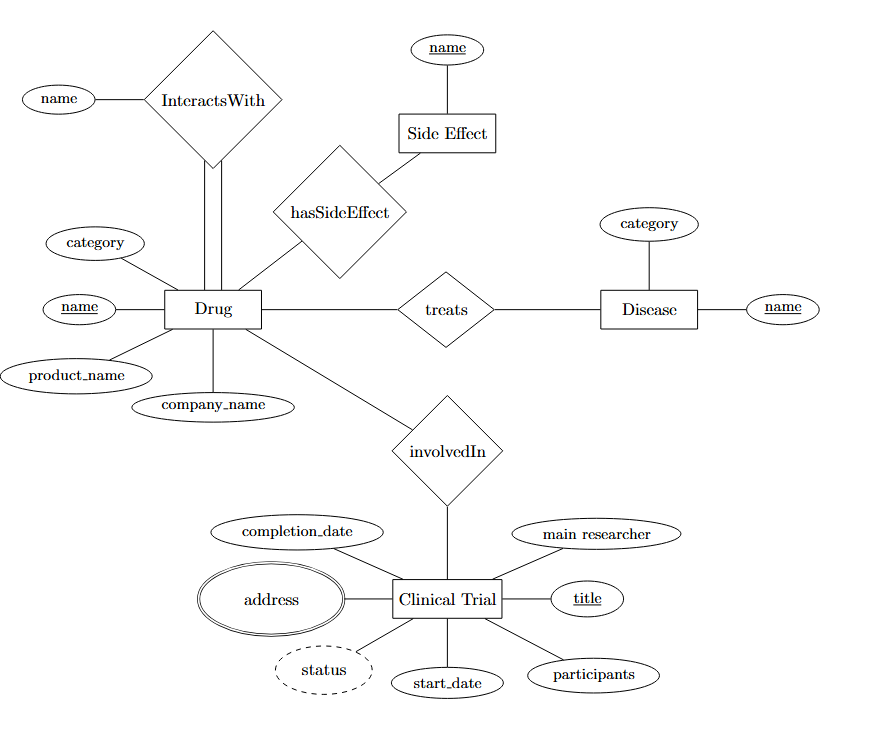
\includegraphics[width=1.2\textwidth]{er (1).png}
    \centering
\end{figure}
\newpage

\section{Relational Model}

This model translates the ER Diagram into a relational schema, specifying tables, attributes, primary keys, foreign keys, and data types with standard professional notation.

\begin{enumerate}
    \item \textbf{Drug}(\underline{drug\_name}, drug\_category, product\_name, company\_name)
    
    \item \textbf{SideEffect}(\underline{name})
    
    \item \textbf{Drug\_hasSideEffect}(\underline{drug\_name}, \underline{side\_effect\_name})
    \begin{itemize}
        \item Foreign key: drug\_name $\longrightarrow$ Drug
        \item Foreign key: side\_effect\_name $\longrightarrow$ SideEffect
    \end{itemize}
    
    \item \textbf{Interaction}(\underline{name})
    
    \item \textbf{Drug\_Interaction}(\underline{drug\_name, interaction\_name})
    \begin{itemize}
        \item Foreign key: drug\_name $\longrightarrow$ Drug
        \item Foreign key: interaction\_name $\longrightarrow$ Interaction
    \end{itemize}
    
    \item \textbf{Disease}(\underline{disease\_name}, disease\_category)
    
    \item \textbf{Treats}(\underline{drug\_name, disease\_name})
    \begin{itemize}
        \item Foreign key: drug\_name $\longrightarrow$ Drug
        \item Foreign key: disease\_name $\longrightarrow$ Disease
    \end{itemize}
    
    \item \textbf{ClinicalTrial}(\underline{clinical\_trial\_title}, clinical\_trial\_start\_date, clinical\_trial\_completion\_date, clinical\_trial\_participants, clinical\_trial\_status, clinical\_trial\_address, clinical\_trial\_institution, clinical\_trial\_address\_1, clinical\_trial\_main\_researcher)
    
    \item \textbf{Drug\_ClinicalTrial}(\underline{drug\_name, clinical\_trial\_title})
    \begin{itemize}
        \item Foreign key: drug\_name $\longrightarrow$ Drug
        \item Foreign key: clinical\_trial\_title $\longrightarrow$ ClinicalTrial
    \end{itemize}
    
\end{enumerate}
\\
\section{Database Implementation}



In this assignment, we are given a sample of medical drug related data. We will use postgreSQL here. Consider the following sample information available  in the given \href{https://docs.google.com/spreadsheets/d/1DBcLdSKGq2FFMarl1Mj08LblRGRgo8IVbphSGerWoiY/edit?gid=1736641593#gid=1736641593}{\textit{Excel file}}.
\subsection{Creating the Database Schema:}
At first, we have to create a database named \testit{DrugSchema}.

\begin{lstlisting}[style=sqlstyle]
create database DrugSchema;
\end{lstlisting}
\subsection{Creating data table:}
\begin{lstlisting}[style=sqlstyle]
CREATE TABLE data (
    drug_name TEXT,
    side_effect TEXT,
    side_effect_1 TEXT,
    side_effect_2 TEXT,
    side_effect_3 TEXT,
    side_effect_4 TEXT,
    interacts_with TEXT,
    interacts_with_1 TEXT,
    interacts_with_2 TEXT,
    disease_name TEXT,
    disease_category TEXT,
    drug_category TEXT,
    product_name TEXT,
    company_name TEXT,
    clinical_trial_title TEXT,
    clinical_trial_start_date TEXT,
    clinical_trial_completion_date TEXT,
    clinical_trial_participants NUMERIC,
    clinical_trial_status TEXT,
    clinical_trial_condition TEXT,
    clinical_trial_condition_1 TEXT,
    clinical_trial_address TEXT,
    clinical_trial_institution TEXT,
    clinical_trial_address_1 TEXT,
    clinical_trial_main_researcher TEXT,
    clinical_trial_condition_2 TEXT
);
\end{lstlisting}
\subsection{Importing Data from CSV into the created data table:}

Let's convert the provided Tutorial1\_data.xlsx file into a CSV format that can be used to populate the database tables. The CSV file's columns will be named according to the tables they correspond to.

\begin{lstlisting}[style=sqlstyle, caption=Run in psql terminal]
COPY data 
FROM 'C:\Users\user\Downloads\Telegram Desktop\Database\Tutorial_1\Tutorial1_data.csv' 
DELIMITER ',' CSV HEADER;
\end{lstlisting}
\newpage 
\section{Create the corresponding tables:}
\begin{lstlisting}[style=sqlstyle]
-- Table for Drug Entity
CREATE TABLE Drug (
    drug_name VARCHAR(255) PRIMARY KEY,
    drug_category VARCHAR(100),
    product_name VARCHAR(255),
    company_name VARCHAR(255)
);

-- Table for SideEffect Entity
CREATE TABLE SideEffect (
    name VARCHAR(255) PRIMARY KEY
);

-- Table for Interaction Entity
CREATE TABLE Interaction (
    name VARCHAR(255) PRIMARY KEY
);

-- Table for Disease Entity
CREATE TABLE Disease (
    disease_name VARCHAR(255) PRIMARY KEY,
    disease_category VARCHAR(100)
);

-- Table for ClinicalTrial Entity (dates as TEXT now)
CREATE TABLE ClinicalTrial (
    clinical_trial_title VARCHAR(500) PRIMARY KEY,
    clinical_trial_start_date TEXT,
    clinical_trial_completion_date TEXT,
    clinical_trial_participants NUMERIC,
    clinical_trial_status VARCHAR(50),
    clinical_trial_address VARCHAR(500),
    clinical_trial_institution VARCHAR(255),
    clinical_trial_address_1 VARCHAR(500),
    clinical_trial_main_researcher VARCHAR(255)
);

-- Table for ClinicalTrialCondition Entity
CREATE TABLE ClinicalTrialCondition (
    name VARCHAR(255) PRIMARY KEY
);

-- Junction Table for Drug-SideEffect relationship
CREATE TABLE Drug_SideEffect (
    drug_name VARCHAR(255) REFERENCES Drug(drug_name) ON DELETE CASCADE,
    side_effect_name VARCHAR(255) REFERENCES SideEffect(name) ON DELETE CASCADE,
    PRIMARY KEY (drug_name, side_effect_name)
);

-- Junction Table for Drug-Interaction relationship
CREATE TABLE Drug_Interaction (
    drug_name VARCHAR(255) REFERENCES Drug(drug_name) ON DELETE CASCADE,
    interaction_name VARCHAR(255) REFERENCES Interaction(name) ON DELETE CASCADE,
    PRIMARY KEY (drug_name, interaction_name)
);

-- Junction Table for Drug-Disease relationship
CREATE TABLE Drug_Disease (
    drug_name VARCHAR(255) REFERENCES Drug(drug_name) ON DELETE CASCADE,
    disease_name VARCHAR(255) REFERENCES Disease(disease_name) ON DELETE CASCADE,
    PRIMARY KEY (drug_name, disease_name)
);

-- Junction Table for Drug-ClinicalTrial relationship
CREATE TABLE Drug_ClinicalTrial (
    drug_name VARCHAR(255) REFERENCES Drug(drug_name) ON DELETE CASCADE,
    clinical_trial_title VARCHAR(500) REFERENCES ClinicalTrial(clinical_trial_title) ON DELETE CASCADE,
    PRIMARY KEY (drug_name, clinical_trial_title)
);

-- Junction Table for ClinicalTrial-Condition relationship
CREATE TABLE ClinicalTrial_Condition (
    clinical_trial_title VARCHAR(500) REFERENCES ClinicalTrial(clinical_trial_title) ON DELETE CASCADE,
    condition_name VARCHAR(255) REFERENCES ClinicalTrialCondition(name) ON DELETE CASCADE,
    PRIMARY KEY (clinical_trial_title, condition_name)
);
\end{lstlisting}
\newpage
\section{Inserting Data into the Database}

Now that we have the data table with all the column from the csv file, we can insert the data into the corresponding tables in our DrugSchema database. Below is the SQL code for every insert statement to populate all the tables.

\begin{lstlisting}[style=sqlstyle]
--Insert into Drug
INSERT INTO Drug (drug_name, drug_category, product_name, company_name)
SELECT DISTINCT drug_name, drug_category, product_name, company_name
FROM data
WHERE drug_name IS NOT NULL
ON CONFLICT (drug_name) DO NOTHING;


-- Insert into SideEffect
INSERT INTO SideEffect (name)
SELECT DISTINCT TRIM(val) AS name
FROM data,
LATERAL UNNEST(ARRAY[
    side_effect, side_effect_1, side_effect_2, side_effect_3, side_effect_4
]) AS val
WHERE val IS NOT NULL AND TRIM(val) <> ''
ON CONFLICT (name) DO NOTHING;


Insert into Interaction
INSERT INTO Interaction (name)
SELECT DISTINCT TRIM(val) AS name
FROM data,
LATERAL UNNEST(ARRAY[
    interacts_with, interacts_with_1, interacts_with_2
]) AS val
WHERE val IS NOT NULL AND TRIM(val) <> ''
ON CONFLICT (name) DO NOTHING;


-- Insert into Disease
INSERT INTO Disease (disease_name, disease_category)
SELECT DISTINCT disease_name, disease_category
FROM data
WHERE disease_name IS NOT NULL
ON CONFLICT (disease_name) DO NOTHING;


-- Insert into ClinicalTrial
INSERT INTO ClinicalTrial (
    clinical_trial_title,
    clinical_trial_start_date,
    clinical_trial_completion_date,
    clinical_trial_participants,
    clinical_trial_status,
    clinical_trial_address,
    clinical_trial_institution,
    clinical_trial_address_1,
    clinical_trial_main_researcher
)
SELECT DISTINCT
    clinical_trial_title,
    clinical_trial_start_date,
    clinical_trial_completion_date,
    clinical_trial_participants,
    clinical_trial_status,
    clinical_trial_address,
    clinical_trial_institution,
    clinical_trial_address_1,
    clinical_trial_main_researcher
FROM data
WHERE clinical_trial_title IS NOT NULL
ON CONFLICT (clinical_trial_title) DO NOTHING;


-- Insert into ClinicalTrialCondition
INSERT INTO ClinicalTrialCondition (name)
SELECT DISTINCT TRIM(val) AS name
FROM data,
LATERAL UNNEST(ARRAY[
    clinical_trial_condition, clinical_trial_condition_1, clinical_trial_condition_2
]) AS val
WHERE val IS NOT NULL AND TRIM(val) <> ''
ON CONFLICT (name) DO NOTHING;


-- Insert into Drug_SideEffect
INSERT INTO Drug_SideEffect (drug_name, side_effect_name)
SELECT DISTINCT drug_name, TRIM(val)
FROM data,
LATERAL UNNEST(ARRAY[
    side_effect, side_effect_1, side_effect_2, side_effect_3, side_effect_4
]) AS val
WHERE drug_name IS NOT NULL AND val IS NOT NULL AND TRIM(val) <> ''
ON CONFLICT (drug_name, side_effect_name) DO NOTHING;


-- Insert into Drug_Interaction
INSERT INTO Drug_Interaction (drug_name, interaction_name)
SELECT DISTINCT drug_name, TRIM(val)
FROM data,
LATERAL UNNEST(ARRAY[
    interacts_with, interacts_with_1, interacts_with_2
]) AS val
WHERE drug_name IS NOT NULL AND val IS NOT NULL AND TRIM(val) <> ''
ON CONFLICT (drug_name, interaction_name) DO NOTHING;


-- Insert into Drug_Disease
INSERT INTO Drug_Disease (drug_name, disease_name)
SELECT DISTINCT drug_name, disease_name
FROM data
WHERE drug_name IS NOT NULL AND disease_name IS NOT NULL
ON CONFLICT (drug_name, disease_name) DO NOTHING;


-- Insert into Drug_ClinicalTrial
INSERT INTO Drug_ClinicalTrial (drug_name, clinical_trial_title)
SELECT DISTINCT drug_name, clinical_trial_title
FROM data
WHERE drug_name IS NOT NULL AND clinical_trial_title IS NOT NULL
ON CONFLICT (drug_name, clinical_trial_title) DO NOTHING;


-- Insert into ClinicalTrial_Condition
INSERT INTO ClinicalTrial_Condition (clinical_trial_title, condition_name)
SELECT DISTINCT clinical_trial_title, TRIM(val)
FROM data,
LATERAL UNNEST(ARRAY[
    clinical_trial_condition, clinical_trial_condition_1, clinical_trial_condition_2
]) AS val
WHERE clinical_trial_title IS NOT NULL AND val IS NOT NULL AND TRIM(val) <> ''
ON CONFLICT (clinical_trial_title, condition_name) DO NOTHING;
\end{lstlisting}
\newpage
\section{Interacting with the Database}

Answering the questions provided in the assignment requires querying the database we just created. Below are the questions and their corresponding SQL queries to retrieve the required information.

\subsection{Question 01}
\textbf{Find the number of drugs that have nausea as a side effect}

Solution:
\begin{lstlisting}[language=SQL]
SELECT COUNT(DISTINCT drug_name) AS drug_count
FROM Drug_SideEffect
WHERE side_effect_name ILIKE 'nausea';
\end{lstlisting}

\subsection{Question 02}
\textbf{Find the drugs that interact with butabarbital}

Solution:
\begin{lstlisting}[language=SQL]
SELECT DISTINCT drug_name
FROM Drug_Interaction
WHERE interaction_name ILIKE 'butabarbital';
\end{lstlisting}

\subsection{Question 03}
\textbf{Find the drugs with side effects cough and headache}

Solution:
\begin{lstlisting}[language=SQL]
SELECT drug_name
FROM Drug_SideEffect
WHERE side_effect_name ILIKE 'cough'
INTERSECT
SELECT drug_name
FROM Drug_SideEffect
WHERE side_effect_name ILIKE 'headache';
\end{lstlisting}

\subsection{Question 04}
\textbf{Find the drugs that can be used to treat endocrine diseases}

Solution:
\begin{lstlisting}[language=SQL]
SELECT DISTINCT drug_name
FROM Drug_Disease
JOIN Disease USING (disease_name)
WHERE disease_category ILIKE 'endocrine%';
\end{lstlisting}

\subsection{Question 05}
\textbf{Find the most common treatment for immunological diseases that have not been used for hematological diseases}

Solution:
\begin{lstlisting}[language=SQL]
SELECT drug_name
FROM Drug_Disease
JOIN Disease USING (disease_name)
WHERE disease_category ILIKE 'immunological'
  AND drug_name NOT IN (
    SELECT drug_name
    FROM Drug_Disease
    JOIN Disease USING (disease_name)
    WHERE disease_category ILIKE 'hematological'
  )
GROUP BY drug_name
ORDER BY COUNT(*) DESC
LIMIT 1;
\end{lstlisting}

\subsection{Question 06}
\textbf{Find the diseases that can be treated with hydrocortisone but not with etanercept}

Solution:
\begin{lstlisting}[language=SQL]
SELECT disease_name
FROM Drug_Disease
WHERE drug_name ILIKE 'hydrocortisone'
EXCEPT
SELECT disease_name
FROM Drug_Disease
WHERE drug_name ILIKE 'etanercept';
\end{lstlisting}

\subsection{Question 07}
\textbf{Find the top-10 side effects that drugs used to treat asthma related diseases have not been used for hematological diseases}

Solution:
\begin{lstlisting}[language=SQL]
SELECT side_effect_name, COUNT(*) AS freq
FROM Drug_SideEffect
WHERE drug_name IN (
    SELECT drug_name
    FROM Drug_Disease
    JOIN Disease USING (disease_name)
    WHERE disease_name ILIKE '%asthma%'
)
AND drug_name NOT IN (
    SELECT drug_name
    FROM Drug_Disease
    JOIN Disease USING (disease_name)
    WHERE disease_category ILIKE 'hematological'
)
GROUP BY side_effect_name
ORDER BY freq DESC
LIMIT 10;
\end{lstlisting}

\subsection{Question 08}
\textbf{Find the drugs that have been studied in more than three clinical trials with more than 30 participants}

Solution:
\begin{lstlisting}[language=SQL]
SELECT drug_name
FROM Drug_ClinicalTrial
JOIN ClinicalTrial USING (clinical_trial_title)
WHERE clinical_trial_participants > 30
GROUP BY drug_name
HAVING COUNT(DISTINCT clinical_trial_title) > 3;
\end{lstlisting}

\subsection{Question 09}
\textbf{Find the largest number of clinical trials and the drugs they have studied that have been active in the same period of time}

Solution:
\begin{lstlisting}[language=SQL]
WITH all_dates AS (
    SELECT clinical_trial_start_date AS date FROM ClinicalTrial
    UNION
    SELECT clinical_trial_completion_date AS date FROM ClinicalTrial
),
active_counts AS (
    SELECT date,
           (SELECT COUNT(*)
            FROM ClinicalTrial
            WHERE clinical_trial_start_date <= date
              AND clinical_trial_completion_date >= date) AS active_trial_count
    FROM all_dates
),
max_date AS (
    SELECT date, active_trial_count
    FROM active_counts
    ORDER BY active_trial_count DESC
    LIMIT 1
),
active_trials_on_max_date AS (
    SELECT clinical_trial_title
    FROM ClinicalTrial
    WHERE clinical_trial_start_date <= (SELECT date FROM max_date)
      AND clinical_trial_completion_date >= (SELECT date FROM max_date)
)
SELECT 
    (SELECT active_trial_count FROM max_date) AS max_active_trials,
    dct.drug_name
FROM Drug_ClinicalTrial dct
JOIN active_trials_on_max_date at ON dct.clinical_trial_title = at.clinical_trial_title;
\end{lstlisting}

\subsection{Question 10}
\textbf{Find the main researchers that have conducted clinical trials that study drugs that can be used to treat both respiratory and cardiovascular diseases}

Solution:
\begin{lstlisting}[language=SQL]
SELECT DISTINCT clinical_trial_main_researcher
FROM ClinicalTrial
JOIN Drug_ClinicalTrial USING (clinical_trial_title)
JOIN Drug_Disease USING (drug_name)
JOIN Disease USING (disease_name)
WHERE disease_category ILIKE 'respiratory'
INTERSECT
SELECT DISTINCT clinical_trial_main_researcher
FROM ClinicalTrial
JOIN Drug_ClinicalTrial USING (clinical_trial_title)
JOIN Drug_Disease USING (drug_name)
JOIN Disease USING (disease_name)
WHERE disease_category ILIKE 'cardiovascular';
\end{lstlisting}

\subsection{Question 11}
\textbf{Find up to three main researchers that have conducted the larger number of clinical trials that study drugs that can be used to treat both respiratory and cardiovascular diseases}

Solution:
\begin{lstlisting}[language=SQL]
WITH both_disease_drugs AS (
  SELECT drug_name
  FROM Drug_Disease
  JOIN Disease USING (disease_name)
  WHERE disease_category ILIKE 'respiratory'
  INTERSECT
  SELECT drug_name
  FROM Drug_Disease
  JOIN Disease USING (disease_name)
  WHERE disease_category ILIKE 'cardiovascular'
),
relevant_trials AS (
  SELECT clinical_trial_main_researcher
  FROM Drug_ClinicalTrial
  JOIN ClinicalTrial USING (clinical_trial_title)
  WHERE drug_name IN (SELECT drug_name FROM both_disease_drugs)
)
SELECT clinical_trial_main_researcher, COUNT(*) AS trial_count
FROM relevant_trials
GROUP BY clinical_trial_main_researcher
ORDER BY trial_count DESC
LIMIT 3;
\end{lstlisting}

\subsection{Question 12}
\textbf{Find the categories of drugs that have been only studied in clinical trials based in United States}

Solution:
\begin{lstlisting}[language=SQL]
SELECT DISTINCT drug_category
FROM Drug
WHERE drug_name IN (
  SELECT drug_name
  FROM Drug_ClinicalTrial
  JOIN ClinicalTrial USING (clinical_trial_title)
  WHERE clinical_trial_address ILIKE '%united states%'
)
AND drug_name NOT IN (
  SELECT drug_name
  FROM Drug_ClinicalTrial
  JOIN ClinicalTrial USING (clinical_trial_title)
  WHERE clinical_trial_address NOT ILIKE '%united states%'
);
\end{lstlisting}


\section{What are the differences to your initial design?}

\subsection{Database Management System Choice}
\begin{itemize}
    \item \textbf{Initial Design:} Planned to use simpler database operations and basic SQL
    \item \textbf{Final Implementation:} Used PostgreSQL with advanced features like \texttt{LATERAL UNNEST} and array handling capabilities
\end{itemize}

\subsection{Data Import Strategy}
\begin{itemize}
    \item \textbf{Initial Design:} Direct insertion from normalized data sources
    \item \textbf{Final Implementation:} Created an intermediate \texttt{data} table to hold raw CSV data, then used complex SQL queries to normalize and populate target tables
\end{itemize}

\subsection{Handling Multiple Values in Single Fields}
\begin{itemize}
    \item \textbf{Initial Design:} Assumed one-to-one relationships for attributes
    \item \textbf{Final Implementation:} Discovered multiple side effects, interactions, and conditions per drug, requiring columns like \texttt{side\_effect\_1}, \texttt{side\_effect\_2}, etc.
\end{itemize}

\subsection{Clinical Trial Entity Complexity}
\begin{itemize}
    \item \textbf{Initial Design:} Simple clinical trial entity with basic attributes
    \item \textbf{Final Implementation:} Added \texttt{ClinicalTrialCondition} as a separate entity with many-to-many relationship through \texttt{ClinicalTrial\_Condition} junction table
\end{itemize}

\subsection{Data Processing Approach}
\begin{itemize}
    \item \textbf{Initial Design:} Basic SQL operations with multiple separate queries for each data type
    \item \textbf{Final Implementation:} Set-based SQL operations using \texttt{LATERAL UNNEST} to handle array-like data efficiently
\end{itemize}

\section{Why did these differences occur?}

\subsection{Real Data Structure Complexity}
The actual CSV data revealed:
\begin{itemize}
    \item Multiple values stored in separate columns (side\_effect, side\_effect\_1, side\_effect\_2, etc.)
    \item Inconsistent data entry requiring \texttt{TRIM()} and \texttt{ILIKE} operations
    \item NULL and empty string handling throughout the dataset
    \item Clinical trial conditions as a separate categorical data requiring normalization
\end{itemize}

\subsection{PostgreSQL Capabilities}
\begin{itemize}
    \item \textbf{Advanced SQL Features:} \texttt{LATERAL UNNEST} allowed elegant handling of multiple columns as arrays
    \item \textbf{Conflict Resolution:} \texttt{ON CONFLICT DO NOTHING} provided robust duplicate handling
    \item \textbf{Array Operations:} PostgreSQL's array handling simplified the normalization process
\end{itemize}

\subsection{Data Quality Challenges}
\begin{itemize}
    \item Discovered inconsistent casing requiring case-insensitive queries (\texttt{ILIKE})
    \item Found whitespace issues necessitating \texttt{TRIM()} functions
    \item Encountered empty strings that needed filtering with \texttt{TRIM(val) <> ''} conditions
\end{itemize}

\subsection{Normalization Requirements}
\begin{itemize}
    \item Multiple side effects per drug required proper many-to-many relationships
    \item Clinical trial conditions needed separate entity modeling
    \item Drug interactions required bidirectional relationship handling
\end{itemize}

\section{What advantages does the new design have over the old one?}

\subsection{Elegant Data Processing}
\begin{lstlisting}[style=sqlcode, caption=PostgreSQL Array Processing vs Row-by-Row Approach]
-- New approach: Process multiple columns as arrays
INSERT INTO SideEffect (name)
SELECT DISTINCT TRIM(val) AS name
FROM data,
LATERAL UNNEST(ARRAY[
    side_effect, side_effect_1, side_effect_2, side_effect_3, side_effect_4
]) AS val
WHERE val IS NOT NULL AND TRIM(val) <> ''
ON CONFLICT (name) DO NOTHING;

-- Old approach would require multiple INSERT statements
-- INSERT INTO SideEffect SELECT DISTINCT side_effect FROM data...
-- INSERT INTO SideEffect SELECT DISTINCT side_effect_1 FROM data...
-- etc.
\end{lstlisting}

\subsection{Robust Data Integrity}
\begin{itemize}
    \item \textbf{Conflict Handling:} \texttt{ON CONFLICT DO NOTHING} prevents duplicate key errors
    \item \textbf{Referential Integrity:} \texttt{ON DELETE CASCADE} maintains consistency
    \item \textbf{Data Validation:} Comprehensive NULL and empty string checking
    \item \textbf{Type Safety:} Proper data types for numeric fields like \texttt{clinical\_trial\_participants}
\end{itemize}

\subsection{Query Performance and Flexibility}
\begin{itemize}
    \item \textbf{Case-Insensitive Searches:} \texttt{ILIKE} operators handle inconsistent data entry
    \item \textbf{Set Operations:} \texttt{INTERSECT}, \texttt{EXCEPT} for complex queries
    \item \textbf{Advanced Joins:} Natural joins using \texttt{USING} clause for cleaner syntax
    \item \textbf{Window Functions:} Support for complex analytical queries
\end{itemize}

\subsection{Scalable Architecture}
\begin{itemize}
    \item \textbf{Modular Design:} Separate entities for each concept (Drug, SideEffect, Interaction, etc.)
    \item \textbf{Junction Tables:} Proper many-to-many relationships with composite primary keys
    \item \textbf{Extensibility:} Easy to add new attributes or entities without breaking existing structure
    \item \textbf{Data Warehousing:} Intermediate \texttt{data} table serves as staging area for ETL processes
\end{itemize}

\subsection{Professional Database Practices}
The final implementation demonstrates:
\begin{itemize}
    \item Proper normalization following 3NF principles
    \item Comprehensive foreign key relationships with appropriate cascade rules
    \item Efficient bulk data loading strategies
    \item Production-ready error handling and data validation
\end{itemize}

\section{Key Insights from Complex Query Implementation}

The tutorial's advanced queries revealed additional design benefits:

\subsection{Complex Analytical Capabilities}
\begin{lstlisting}[style=sqlcode, caption=Advanced Query Example]
-- Finding drugs treating both respiratory AND cardiovascular diseases
SELECT drug_name
FROM Drug_Disease
JOIN Disease USING (disease_name)
WHERE disease_category ILIKE 'respiratory'
INTERSECT
SELECT drug_name
FROM Drug_Disease
JOIN Disease USING (disease_name)
WHERE disease_category ILIKE 'cardiovascular';
\end{lstlisting}

\subsection{Time-Based Analysis Support}
The clinical trial date handling supports complex temporal queries for finding overlapping trials and active research periods, demonstrating the database's capability for longitudinal medical research analysis.

The transformation from initial design to final implementation taught several crucial database development principles:

\begin{itemize}
    \item \textbf{Data Exploration First:} Always examine actual data before finalizing schema design.
    \item \textbf{Staged Implementation:} Using intermediate tables for complex data transformations.
    \item \textbf{PostgreSQL Power:} Advanced SQL features can dramatically simplify complex data processing.
    \item \textbf{Normalization Benefits:} Proper entity separation enables sophisticated analytical queries.
    \item \textbf{Error Handling:} Production databases require comprehensive conflict resolution strategies.
\end{itemize}




\end{document}
